\documentclass[hidelinks,12pt]{article}
\usepackage[left=0.25cm,top=1cm,right=0.25cm,bottom=1cm]{geometry}
%\usepackage[landscape]{geometry}
\textwidth = 20cm
\hoffset = -1cm
\usepackage[utf8]{inputenc}
\usepackage[spanish,es-tabla]{babel}
\usepackage[autostyle,spanish=mexican]{csquotes}
\usepackage[tbtags]{amsmath}
\usepackage{nccmath}
\usepackage{amsthm}
\usepackage{amssymb}
\usepackage{mathrsfs}
\usepackage{graphicx}
\usepackage{subfig}
\usepackage{standalone}
\usepackage[outdir=./Imagenes/]{epstopdf}
\usepackage{siunitx}
\usepackage{physics}
\usepackage{color}
\usepackage{float}
\usepackage{hyperref}
\usepackage{multicol}
%\usepackage{milista}
\usepackage{anyfontsize}
\usepackage{anysize}
%\usepackage{enumerate}
\usepackage[shortlabels]{enumitem}
\usepackage{capt-of}
\usepackage{bm}
\usepackage{relsize}
\usepackage{placeins}
\usepackage{empheq}
\usepackage{cancel}
\usepackage{wrapfig}
\usepackage[flushleft]{threeparttable}
\usepackage{makecell}
\usepackage{fancyhdr}
\usepackage{tikz}
\usepackage{bigints}
\usepackage{scalerel}
\usepackage{pgfplots}
\usepackage{pdflscape}
\pgfplotsset{compat=1.16}
\spanishdecimal{.}
\renewcommand{\baselinestretch}{1.5} 
\renewcommand\labelenumii{\theenumi.{\arabic{enumii}})}
\newcommand{\ptilde}[1]{\ensuremath{{#1}^{\prime}}}
\newcommand{\stilde}[1]{\ensuremath{{#1}^{\prime \prime}}}
\newcommand{\ttilde}[1]{\ensuremath{{#1}^{\prime \prime \prime}}}
\newcommand{\ntilde}[2]{\ensuremath{{#1}^{(#2)}}}

\newtheorem{defi}{{\it Definición}}[section]
\newtheorem{teo}{{\it Teorema}}[section]
\newtheorem{ejemplo}{{\it Ejemplo}}[section]
\newtheorem{propiedad}{{\it Propiedad}}[section]
\newtheorem{lema}{{\it Lema}}[section]
\newtheorem{cor}{Corolario}
\newtheorem{ejer}{Ejercicio}[section]

\newlist{milista}{enumerate}{2}
\setlist[milista,1]{label=\arabic*)}
\setlist[milista,2]{label=\arabic{milistai}.\arabic*)}
\newlength{\depthofsumsign}
\setlength{\depthofsumsign}{\depthof{$\sum$}}
\newcommand{\nsum}[1][1.4]{% only for \displaystyle
    \mathop{%
        \raisebox
            {-#1\depthofsumsign+1\depthofsumsign}
            {\scalebox
                {#1}
                {$\displaystyle\sum$}%
            }
    }
}
\def\scaleint#1{\vcenter{\hbox{\scaleto[3ex]{\displaystyle\int}{#1}}}}
\def\bs{\mkern-12mu}


\title{Asesoría Repaso Tema 1 \vspace{-1ex}}
\author{M. en C. Gustavo Contreras Mayén}
\date{ }
\newcommand{\Cancel}[2][black]{{\color{#1}\cancel{\color{black}#2}}}
\begin{document}
\vspace{-4cm}
\maketitle
\fontsize{14}{14}\selectfont
\tableofcontents
\newpage


\section{Funciones Gamma y Beta}
\subsection{Repaso de las funciones}


En la parte del curso en donde trabajamos con las funciones Gamma y Beta, se presentó la definición de cada una de ellas en términos de una integral: la función Gamma para cualquier $p >0$, es:
\begin{align*}
\Gamma (p) = \int_{0}^{\infty} x^{p-1} \, e^{-x} \dd{x}, \hspace{1cm} p > 0
\end{align*}

Mientras que la función Beta: 
\begin{align*}
\begin{gathered}
B(p, q) = \int_{0}^{1} x^{p-1} \, (1- x )^{q-1} \dd{x}, \\
\mbox{con }  p > 0, q > 0
\end{gathered}
\end{align*}

Posteriormente se revisaron algunas de las propiedades tanto para la función Gamma como para la función Beta, se realizó la demostración de esas propiedades (no todas), a partir de la definición de las funciones.

\par
Se revisó también una relación entre la función Beta y Gamma, que nos permite entonces obtener un valor ya sea en términos de factores de $\sqrt{\pi}$ o en su caso, un valor númerico.
\par
En física encontraremos estas funciones en desarrollos que involucran el manejo de los factoriales, es por ello que nos conviene su uso.
\par
También serán de utilidad para resolver algunas integrales que en apariencia son complicadas, aprovechando las propiedades de ambas funciones.

\section{Resolviendo integrales}
\subsection{Ejercicio 1}

\textbf{Ejercicio 1 -  Enunciado: } Calcula el área $A$ encerrada entre el eje $x$ y un arco de la curva $y = \sin^{8} x$ en el intervalo $[0, \pi]$.
\par
Lo que se nos pide es calcular el área debajo de la curva que se muestra a continuación:
\begin{figure}[H]
    \centering
    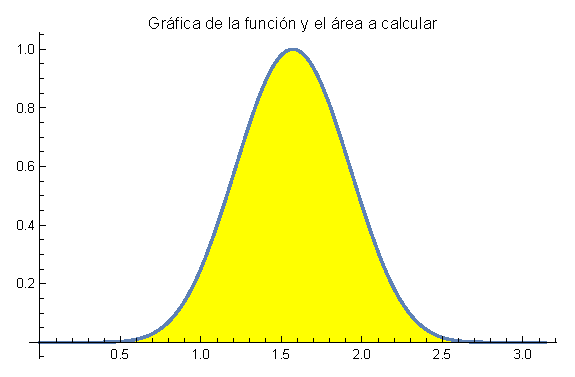
\includegraphics[scale=0.9]{Imagenes/Asesoria_03_01.eps}
\end{figure}

Sabemos por el curso de Cálculo II, que el área debajo de la curva la podemos obtener resolviendo la integral:
\begin{align*}
A = \int_{0}^{\pi} \sin^{8} x \dd{x}
\end{align*}

De entrada la integral no se mira amigable como para usar alguna identidad trigonométrica o algún cambio de variable tan inmediato.

\par
Con la finalidad de simplificar la expresión, vemos de la gráfica anterior, que podemos calcular la integral (y por lo tanto, conocer el área $A$), al reducir el intervalo de integración, aprovechando la simetría de la curva:
\begin{align*}
A = 2 \int_{0}^{\frac{\pi}{2}} \sin^{8} x \dd{x}
\end{align*}

El integrando de interés lo podemos multiplicar por un $1$ en particular: $\cos^{0} x$, de tal manera que quede expresado como:
\begin{align*}
A = 2 \int_{0}^{\frac{\pi}{2}} \sin^{8} x \cos^{0} x \dd{x}
\end{align*}

que podemos dejar como:
\begin{align*}
A = \int_{0}^{\frac{\pi}{2}} 2 \, \sin^{8} x \cos^{0} x \dd{x}
\end{align*}

Si hacemos el cambio de variable $x = \theta$, llegamos a:
\begin{align*}
A = \int_{0}^{\frac{\pi}{2}} 2 \, \sin^{8} \theta \cos^{0} \theta \dd{\theta}
\end{align*}

Por lo que podemos usar la identidad:
\begin{align*}
B(x, y) = \int_{0}^\frac{\pi}{2} 2 \, \sin^{2x-1} \theta \, \cos^{2y-1} \theta \dd{\theta}
\end{align*}

Entonces tendremos que:
\begin{align*}
2 \, x - 1 = 8 &\Rightarrow x = \dfrac{9}{2} \\[0.5em]
2 \, y - 1 = 0 &\Rightarrow y = \dfrac{1}{2}
\end{align*}

Por lo que la integral pasa a ser:
\begin{align*}
A = B \left( \dfrac{9}{2},\dfrac{1}{2} \right)
\end{align*}

Nos queda entonces obtener el valor de la función Beta con los argumentos dados, y tendremos entonces el valor del área solicitado.
\par
Ocuparemos una relación entre las funciones Gamma y Beta, y entonces evaluar la función Gamma para obtener dicho valor del área.
\par
Sabemos que:
\begin{align*}
B (x, y) = \dfrac{\Gamma (x) \, \Gamma (y)}{\Gamma (x + y)}
\end{align*}

Entonces:
\begin{align*}
A &= B \left( \dfrac{9}{2},\dfrac{1}{2} \right) = \dfrac{\Gamma \left(\dfrac{9}{2} \right) \, \Gamma \left(\dfrac{1}{2} \right)}{\Gamma \left(\dfrac{9}{2} + \dfrac{1}{2} \right)}
\end{align*}

Obtenemos los valores de la función Gamma:
\begin{align*}
\Gamma \left( \dfrac{1}{2} \right) &= \sqrt{\pi} \\[0.5em] 
\Gamma \left( \dfrac{9}{2} + \dfrac{1}{2} \right) &= \Gamma (5) = (5 - 1)! = 4! = 24 \\[0.5em] 
\Gamma \left(n + \dfrac{1}{2}\right) &= \dfrac{1 \cdot 3 \cdot 5 \ldots (2 \, n - 1)}{2^{n}} \, \sqrt{\pi} 
\end{align*}

Para el último valor, se tiene que:
\begin{align*}
\Gamma \left( \dfrac{9}{2}\right) &=  \Gamma \left(4 + \dfrac{1}{2}\right) = \dfrac{1 \cdot 3 \cdot 5 \cdot (2 \cdot 4 - 1)}{2^{4}} \, \sqrt{\pi} \\[1em]
&= \dfrac{105 \sqrt{\pi}}{16}
\end{align*}

Tendremos entonces que el valor del área es:
\begin{align*}
A &= \dfrac{\dfrac{105 \sqrt{\pi}}{16} \, \sqrt{\pi}}{24} = \\[0.5em]
&= \dfrac{105 \sqrt{\pi}}{384} = \\[0.5em]
&= \dfrac{35 \, \pi}{128} \qed
\end{align*}

\subsection{Ejercicio 2}

\textbf{Enunciado: } Calcula el área $A$ encerrada en el óvalo definido por:
\begin{align*}
y^{2} = \dfrac{1 - x^{2}}{1 + x^{2}}
\end{align*}

Un paso que se recomienda siempre, es el de contar con una referencia gráfica de la función que se nos presenta.
\par
Para ello ocupamos cualquier programa que nos genere la gráfica:
\begin{figure}[H]
    \centering
    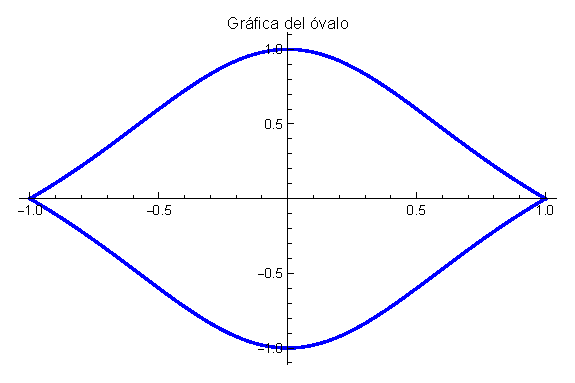
\includegraphics[scale=1]{Imagenes/Asesoria_03_02.eps}
\end{figure}

Observamos que esta curva está limitada por las líneas $x \pm 1$, ya que $y^{2}$ sería negativo para $\abs{x} > 1$.
\par
De manera similar, al resolver para $x^{2}$, se encuentra que la curva está limitada por las líneas $y = \pm 1$. La restricción sobre $x$ sugiere un cambio de variable.
\par
Sea el cambio de variable:
\begin{align*}
x^{2} = \sin t \hspace{0.2cm} \Rightarrow \hspace{0.2cm} \dd{x} = \dfrac{1}{2} \dfrac{\cos t}{\sqrt{\sin t}} \dd{t}
\end{align*}

Adicionalmente tenemos que la curva es simétrica en ambos ejer coordenados, por lo que podemos calcular el área en el primer cuadrante y multiplicar por $4$ para obtener el área total.

\begin{figure}[H]
    \centering
    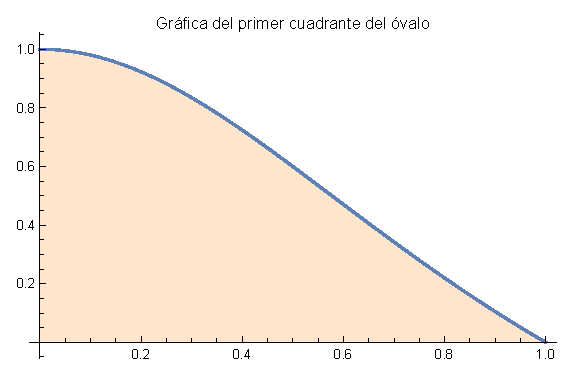
\includegraphics[scale=1]{Imagenes/Asesoria_03_03.eps}
\end{figure}

Tenemos entonces que:
\begin{align*}
A = 4 \int_{0}^{1} y \dd{x} =  4 \int_{0}^{\frac{\pi}{2}} \sqrt{{\dfrac{1 - \sin t}{1 + \sin t}}} \, \cdot \dfrac{1}{2} \, \dfrac{\cos t}{\sqrt{\sin t}} \dd{t}
\end{align*}

Que nuevamente aparenta complicar más el integrando, pero recurrimos al álgebra para intentar simplificarlo:

Si multiplicamos el radical del integrando por un $1 = 1 - \sin t / 1 - \sin t$, tendremos:
\begin{align*}
A &= 2 \int_{0}^{\frac{2}{\pi}} \sqrt{\dfrac{(1 - \sin t)^{2}}{\cos^{2} t}} \, \dfrac{\cos t}{\sqrt{\sin t}} \dd{t} = \\[1em]
&= 2 \int_{0}^{\frac{\pi}{2}} \big( \sin^{-\frac{1}{2}} t - \sin^{\frac{1}{2}} t \big) \dd{t} = \\[1em]
&= 2 \int_{0}^{\frac{\pi}{2}} \dfrac{\dd{t}}{\sin^{\frac{1}{2}} \, t} - 2 \int_{0}^{\frac{\pi}{2}} \sin^{\frac{1}{2}} t \dd{t}
\end{align*}

La segunda de estas dos integrales es propia, pero la primera es impropia.
\par
Sabemos que \emph{la integral impropia debe ser convergente} porque sabemos que el área $A$ es finita, ya que $A$ está completamente contenida dentro de un cuadrado de lado 2.
\par
Veamos la convergencia de la integral impropia.

La razón $t/\sin t \to 1$ cuando en el límite $t \to 0$. Esto hace que el integrando sea \enquote{similar} a $1 / t^{1/2}$ mientras $t \to 0$, con la consecuencia de que la convergencia de la integral:
\begin{align*}
\int_{0}^{\frac{\pi}{2}} \dfrac{\dd{t}}{\sin^{\frac{1}{2}} \, t}
\end{align*}
depende ya sea de la convergencia o divergencia de:
\begin{align*}
\int_{0}^{\frac{\pi}{2}} \dfrac{\dd{t}}{t^{\frac{1}{2}}}
\end{align*}

Pero sabemos que esta última integral es convergente porque el exponente en $t$ es menor que la unidad. Por tanto, la integral en cuestión también es convergente.
\par
Ahora insertamos el factor $\cos^{0} t$ que nos permite reconocer las integrales como integrales Beta:
\begin{align*}
A = \int_{0}^{\frac{\pi}{2}} 2 \sin^{-\frac{1}{2}} t \cos^{0} t \dd{t} - \int_{0}^{\frac{\pi}{2}} 2 \sin^{\frac{1}{2}} t \cos^{0} t \dd{t}
\end{align*}

Por la identidad anteriormente utilizada:
\begin{align*}
A = B \left( \dfrac{1}{4}, \dfrac{1}{2} \right) - B \left( \dfrac{3}{4}, \dfrac{1}{2} \right)
\end{align*}

Tenemos entonces que calcular:
\begin{align*}
A = \dfrac{\sqrt{\pi} \, \Gamma \left( \dfrac{1}{4} \right)}{\Gamma \left( \dfrac{3}{4} \right)} - \dfrac{\sqrt{\pi} \, \Gamma \left( \dfrac{3}{4} \right)}{\Gamma \left( \dfrac{5}{4} \right)}
\end{align*}

Haciendo las respectivas operaciones para evaluar las funciones Gamma con los argumentos, y simplificando con un valor numérico (que se puede obtener mediante el uso de software matemático o de programación), tenemos que el área $A$ en cerrada en el óvalo inicial es:

\begin{align*}
A = 2.847
\end{align*}
\end{document}